\documentclass{article}

% Symbols
\usepackage{recycle}
\usepackage{amsfonts, amsthm}
\usepackage{upgreek}
\usepackage{physics}
\usepackage{cancel}
\usepackage{amssymb, latexsym, amsmath}

% Proof
\renewcommand*{\proofname}{\textbf{Demostraci\'on:}}

% Graphics
\usepackage{graphicx}
\usepackage{pgf}

% Color a letras.
%\usepackage[usenames,dvipsnames,svgnames,table]{xcolor}

% Tikz
\usepackage{tikz}
\usetikzlibrary{arrows,automata}
\usepackage{tikz}
\usetikzlibrary{arrows,automata}

\usetikzlibrary{shapes,calc}
\tikzstyle{edge}=[shorten <=2pt, shorten >=2pt,
  >=stealth, line width=1.1pt]
\tikzstyle{blueE}=[shorten <=2pt, shorten >=2pt,
  >=stealth, line width=1.5pt, blue]
\tikzstyle{blackV}=[circle, fill=black,
  minimum size=6pt,
  inner sep=0pt, outer sep=0pt]
\tikzstyle{blueV}=[circle, fill=blue, draw,
  minimum size=6pt, line width=0.75pt,
  inner sep=0pt, outer sep=0pt]
\tikzstyle{redV}=[circle, fill=red, draw,
  minimum size=6pt, line width=0.75pt,
  inner sep=0pt, outer sep=0pt]
\tikzstyle{redSV}=[semicircle, fill=red, minimum
  size=3pt, inner sep=0pt, outer sep=0pt,
  rotate=225]
\tikzstyle{blueSV}=[semicircle, fill=blue, minimum
  size=3pt, inner sep=0pt, outer sep=0pt,
  rotate=225]
\tikzstyle{blackSV}=[semicircle, fill=black, minimum
  size=3pt, inner sep=0pt, outer sep=0pt,
  rotate=225]
\tikzstyle{vertex}=[circle, draw, minimum size=6pt,
  line width=0.75pt, inner sep=0pt,
  outer sep=0pt]

% Margins
\addtolength{\voffset}{-1cm}
\addtolength{\hoffset}{-1.5cm}
\addtolength{\textwidth}{3cm}
\addtolength{\textheight}{2cm}

%Header-Footer
\usepackage{fancyhdr}
\renewcommand{\headrulewidth}{1pt}

\newcommand{\set}[1]{%
  \left\{ #1 \right\}%
}

\pagenumbering{gobble}
\footskip = 50pt
\renewcommand{\headrulewidth}{1pt}

\pagestyle{fancyplain}

\begin{document}
\title{UNIVERSIDAD AUT\'ONOMA DE M\'EXICO\\ Facultad de Ciencias}
\author{Autores:
  \\ Fernanda Villaf\'an Flores
  \\ Fernando Alvarado Palacios
  \\ Adri\'an Aguilera Moreno}
\date{}
\maketitle
\begin{center}
  
\includegraphics[scale=0.20]{../Imagen/Portada.jpg}\\[0.4cm]
  \Large
  \bf{Gr\'aficas y Juegos}
  \normalsize
\end{center}
\newpage
\fancyhead[r]{ Gr\'aficas y Juegos 2022-1}
\section*{\LARGE{Tarea 1}}

\begin{enumerate}
  %%%%%%%%%%%%%%%%%%%%%%%%%%%%%%%%% 1 %%%%%%%%%%%%%%%%%%%%%%%%%%%%%%%%%%%%%%%%%%%
  \item Sea $n$ un entero, $n \ge 3$. Demuestre que existe un \'unico
    $n$-ciclo, salvo isomorfismo.
    \renewcommand\qedsymbol{QED}
    \begin{proof}
      Sean $G$ y $H$ ciclos de orden $n$.

      Tomamos $V_{G} = (v_{1}, \dotsm, v_{n}, v_{1})$ y
      $V_{H} = (v_{1}, \dotsm, v_{n}, v_{1})$.

      Como $G$ y $H$ son ciclos, sabemos que son $2$-regular. \\
      Es decir, podemos suponer que un v\'ertice $v_{i}$ de $G$
      con $i \in  \{1, \dotsm, n\}$ es adyacente a dos v\'ertices
      (digamos $v_{i - 1}$ y $v_{i + 1}$). Notemos que $v_{1} = v_{n}$. \\
      An\'alogamente para $H$.

      Ahora, como $G$ y $H$ son de orden $n$, definimos una
      funci\'on $\phi: V_{G} \rightarrow V_{H}$ dada por
      $\phi(v_{i}) = u_{i}$ para cada $i \in  \{1, \dotsm, n\}$.

      Claramente $\phi$ es una biyecci\'on.

      Demostraremos que $\phi$ es un isomorfismo:
      \begin{itemize}
      \item[$\Rightarrow$)] Si $v_{i} v_{j} \in E_{G}$, entonces
        podemos suponer, sin p\'erdida de generalidad, que $j = i + 1$ o $j = i -1$.

        Por definici\'on de $\phi$, tenemos que $\phi(v_{i}) = u_{i}$
        y $\phi(v_{j}) = u_{j} = u_{i + 1}$ (an\'alogamente cuando $j = i - 1$).

        Como $u_{i}u_{j} = u_{i}u_{i + 1} \in E_{H}$, concluimos que
        $\phi(v_{i})\phi(v_{j}) \in E_{H}$.
      \item[$\Leftarrow$)] Reciprocamente, si $v_{i} v_{j} \notin E_{G}$,
        entonces $j \neq i+1$ y $j \neq i-1$.

        Se sigue que $\phi (v_{i}) \phi (v_{j}) = u_{i} u_{j} \notin E_{H}$.
      \end{itemize}

      Por lo tanto, demostramos que existe un \'unico $n$-ciclo
      (salvo isomorfismo).
    \end{proof}

  %%%%%%%%%%%%%%%%%%%%%%%%%%%%%%%%% 2 %%%%%%%%%%%%%%%%%%%%%%%%%%%%%%%%%%%%%%%%%%%
  \item De un ejemplo de tres gr\'aficas del mismo orden, mismo tama\~no y misma
    sucesi\'on de grados tales que cualesquiera dos de dichas gr\'aficas no sean
    isomorfas, al menos una de ellas sea conexa, y al menos una sea inconexa.

    A continuaci\'on se muestran las gr\'aficas: $G_1, G_2$ y $G_3$:

    \begin{figure}[ht!]
      \centering
      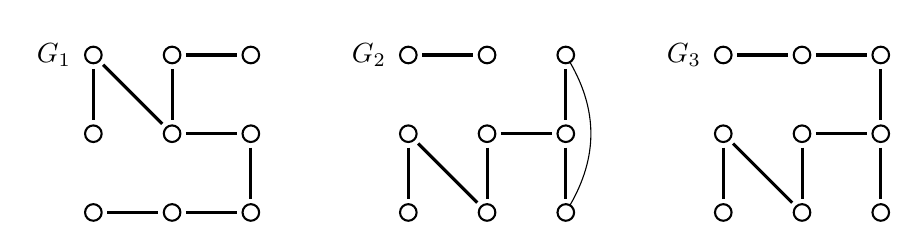
\begin{tikzpicture}
        %%%%%  Componente izquierda  %%%%%
        \node (0) [vertex,label=180:] at (0,1){};
        \node (1) [vertex,label=90:]  at (1,1){};
        \node (2) [vertex,label=90:]  at (2,1){};
        \node (3) [vertex,label=90:]  at (0,0){};
        \node (4) [vertex,label=90:]  at (1,0){};
        \node (5) [vertex,label=90:]  at (2,0){};
        \node (6) [vertex,label=90:]  at (0,-1){};
        \node (7) [vertex,label=90:]  at (1,-1){};
        \node (8) [vertex,label=90:]  at (2,-1){};

        \draw [edge] (0) to (3);
        \draw [edge] (0) to (4);
        \draw [edge] (1) to (4);
        \draw [edge] (1) to (2);
        \draw [edge] (4) to (5);
        \draw [edge] (5) to (8);
        \draw [edge] (6) to (7);
        \draw [edge] (7) to (8);

        \node (L) at (-0.5,1){$G_1$};

        %%%%% Componente derecha  %%%%%
        \begin{scope}[xshift=4cm]
          \node (9) [vertex,label=180:]  at (0,1){};
          \node (10) [vertex,label=90:]  at (1,1){};
          \node (11) [vertex,label=90:]  at (2,1){};
          \node (12) [vertex,label=90:]  at (0,0){};
          \node (13) [vertex,label=90:]  at (1,0){};
          \node (14) [vertex,label=90:]  at (2,0){};
          \node (15) [vertex,label=90:]  at (0,-1){};
          \node (16) [vertex,label=90:]  at (1,-1){};
          \node (17) [vertex,label=90:]  at (2,-1){};

          \draw [edge] (9)  to (10);
          \draw [edge] (11) to (14);
          \draw [edge] (12) to (16);
          \draw [edge] (12) to (15);
          \draw [edge] (13) to (14);
          \draw [edge] (13) to (16);
          \draw [edge] (14) to (17);
          \path(11)edge[bend left]node{}(17);
          \node (L) at (-0.5,1){$G_2$};
        \end{scope}

        %%%%% Componente debajo  %%%%%%
        \begin{scope}[xshift=8cm]
          \node (0) [vertex,label=180:] at (0,1){};
          \node (1) [vertex,label=90:]  at (1,1){};
          \node (2) [vertex,label=90:]  at (2,1){};
          \node (3) [vertex,label=90:]  at (0,0){};
          \node (4) [vertex,label=90:]  at (1,0){};
          \node (5) [vertex,label=90:]  at (2,0){};
          \node (6) [vertex,label=90:]  at (0,-1){};
          \node (7) [vertex,label=90:]  at (1,-1){};
          \node (8) [vertex,label=90:]  at (2,-1){};

          \draw [edge] (0) to (1);
          \draw [edge] (1) to (2);
          \draw [edge] (2) to (5);
          \draw [edge] (3) to (6);
          \draw [edge] (3) to (7);
          \draw [edge] (4) to (5);
          \draw [edge] (4) to (7);
          \draw [edge] (5) to (8);

          \node (L) at (-0.5,1){$G_3$};
        \end{scope}
      \end{tikzpicture}
    \end{figure}

  %  \begin{figure}[ht!]
  %    \centering
  %    \begin{tikzpicture}
  %
  %      \node (0) [vertex,label=180:] at (0,1){};
  %      \node (1) [vertex,label=90:]  at (1,1){};
  %      \node (2) [vertex,label=90:]  at (2,1){};
  %      \node (3) [vertex,label=90:]  at (0,0){};
  %      \node (4) [vertex,label=90:]  at (1,0){};
  %      \node (5) [vertex,label=90:]  at (2,0){};
  %      \node (6) [vertex,label=90:]  at (0,-1){};
  %      \node (7) [vertex,label=90:]  at (1,-1){};
  %      \node (8) [vertex,label=90:]  at (2,-1){};
  %
  %      \draw [edge] (0) to (1);
  %      \draw [edge] (1) to (2);
  %      \draw [edge] (2) to (5);
  %      \draw [edge] (3) to (6);
  %      \draw [edge] (3) to (7);
  %      \draw [edge] (4) to (5);
  %      \draw [edge] (4) to (7);
  %      \draw [edge] (5) to (8);
  %
  %      \node (L) at (-0.5,1){$G_3$};
  %    \end{tikzpicture}
  %  \end{figure}

    con sucesiones orden $9$, tamaño $8$ y sucesi\'on de grados $(1,1,1,2,2,2,2,2,3)$.
    \hfill $\square$

  %%%%%%%%%%%%%%%%%%%%%%%%%%%%%%%%% 3 %%%%%%%%%%%%%%%%%%%%%%%%%%%%%%%%%%%%%%%%%%%
  \item Sea $D$ una digr\'afica.   Demuestre que
  $$\sum_{v \in V_D} d^+(v) = \sum_{v \in V_D} d^-(v) = |A_D|.$$

    \renewcommand\qedsymbol{QED}
    \begin{proof}
      La demostraci\'on se dividir\'a en dos incisos:
      \begin{itemize}
        \item[$\cdot$)] $\displaystyle \sum_{v \in V_{D}} d^{+}(v) = \abs{A_{D}}$

          Sea $M_{1}$ una matriz de incidencia de $D$, tal que:
          \begin{center}
            $M_{1} = M^{+}_{ij}
            = \left \{
            \begin{array}{lcc}
              1 &   si  & v_{i} \hspace{0.3em} es \hspace{0.3em} la
              \hspace{0.3em} cola \hspace{0.3em} de \hspace{0.3em} e_{j} \\
              \\0 &  si & v_{i} \hspace{0.3em} no \hspace{0.3em} es \hspace{0.3em}
              la \hspace{0.3em} cola \hspace{0.3em} de \hspace{0.3em} e_{j}
            \end{array}
            \right.$
          \end{center}
          Ahora, supongamos que $V = \{v_{1}, \dotsm, v_{n}\}$ donde $v_{i}$
          corresponde al \textit{i-\'esimo} rengl\'on de $M_{1}$.

          Sabemos que las entradas de cada columna de $M_{1}$ son igual a 1,
          que son las flechas $e_{j}$ con un v\'ertice llamado \textit{cola de la flecha}.
          Por otro lado, las entradas del \textit{i-\'esimo} rengl\'on de $M_{1}$
          suman $d^{+}(v_{i})$, ya que las entradas corresponden a todas las
          flechas de las cuales $v_{i}$ es cola de dicha flecha.

          Entonces, tenemos que:
          \begin{equation*}
            \begin{split}
              \abs{A_{D}} & = \sum_{j=1}^{\abs{A}} \sum_{i=1}^{\abs{V}} M^{+}_{ij} \\
              & = \sum_{i=1}^{\abs{V}} \sum_{j=1}^{\abs{A}} M^{+}_{ij} \\
              & = \sum_{i=1}^{\abs{V}} d^{+}(v_{i}) \\
              & = \sum_{v \in V} d^{+}(v)
            \end{split}
          \end{equation*}
          De forma an\'aloga se realiza el otro inciso.

        \item[$\cdot\cdot$)] $\displaystyle \sum_{v \in V_{D}} d^{-}(v) = \abs{A_{D}}$

          Sea $M_{2}$ una matriz de incidencia de $D$, tal que:
          \begin{center}
            $M_{2} = M^{-}_{ij}
            = \left \{
            \begin{array}{lcc}
              1 &   si  & v_{i} \hspace{0.3em} es \hspace{0.3em} la \hspace{0.3em}
              cabeza \hspace{0.3em} de \hspace{0.3em} e_{j} \\
              \\0 &  si & v_{i} \hspace{0.3em} no \hspace{0.3em} es \hspace{0.3em}
              la \hspace{0.3em} cabeza \hspace{0.3em} de \hspace{0.3em} e_{j}
            \end{array}
            \right.$
          \end{center}
          Ahora, supongamos que $V = \{v_{1}, \cdots, v_{n}\}$ donde $v_{i}$
          corresponde al \textit{i-\'esimo} rengl\'on de $M_{1}$.

          Sabemos que las entradas de cada columna de $M_{1}$ son igual a 1,
          que son las flechas $e_{j}$ con un v\'ertice llamado \textit{cabeza de la flecha}.
          Por otro lado, las entradas del \textit{i-ésimo} rengl\'on de $M_{1}$
          suman $d^{-}(v_{i})$, ya que las entradas corresponden a todas las
          flechas de las cuales $v_{i}$ es cabeza de dicha flecha.

          Entonces, tenemos que:
          \begin{equation*}
            \begin{split}
              \abs{A_{D}} & = \sum_{j=1}^{\abs{A}} \sum_{i=1}^{\abs{V}} M^{-}_{ij} \\
              & = \sum_{i=1}^{\abs{V}} \sum_{j=1}^{\abs{A}} M^{-}_{ij} \\
              & = \sum_{i=1}^{\abs{V}} d^{-}(v_{i}) \\
              & = \sum_{v \in V} d^{-}(v)
            \end{split}
          \end{equation*}
      \end{itemize}
      Por lo tanto, queda demostrado que:
      \[
      \displaystyle \sum_{v \in V_D} d^+(v) = \sum_{v \in V_D} d^-(v) = |A_D|
      \]
    \end{proof}

  %%%%%%%%%%%%%%%%%%%%%%%%%%%%%%%%% 4 %%%%%%%%%%%%%%%%%%%%%%%%%%%%%%%%%%%%%%%%%%%
  \item  Sea $n$ un entero positivo. Definimos a la {\em Ret\'icula Booleana},
  $BL_n$, como la gr\'afica cuyo conjunto de vértices es el conjunto de todos
  los posibles subconjuntos de $\set{1, \cdots, n}$, donde dos subconjuntos
  $X$ y $Y$ son adyacentes si y s\'olo si su diferencia sim\'etrica tiene
  exactamente un elemento.

    \begin{enumerate}
      \item Dibuje $BL_1, BL_2, BL_3$ y $BL_4$.

        %-------------------------- inciso (a) ---------------------
        %~~~~~~~~~~~~~~~~~~~~~~~~~~~~~~~~~~~~~~~~~~ BL_1
        Gr\'afica representativa de $BL_1$:
        \begin{center}
          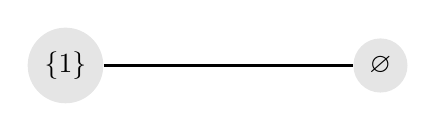
\begin{tikzpicture}
            \tikzstyle{vertex} = [circle, fill = black!10]
            \tikzstyle{edge}   = [-, thick]

            \node[vertex](v1)  at (0,0)  {$\{1\}$};
            \node[vertex](v2)  at (4,0)  {$\varnothing$};
            %%------------ Aristas ---------
            \draw[edge](v1)--(v2);
          \end{tikzpicture}
        \end{center}

        %~~~~~~~~~~~~~~~~~~~~~~~~~~~~~~~~~~~~~~~~~~ BL_2
        Gr\'afica representativa de $BL_2$:
        \begin{center}
          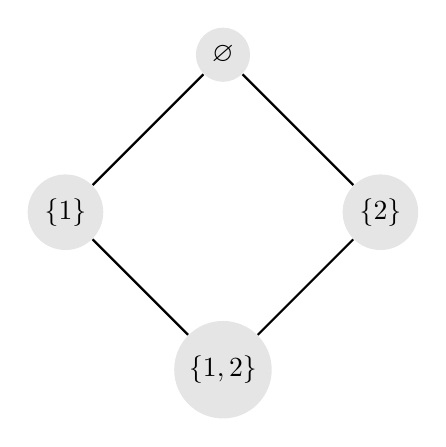
\begin{tikzpicture}
            \tikzstyle{vertex} = [circle, fill = black!10]
            \tikzstyle{edge}   = [-, thick]

            \node[vertex](v1)  at (0,2)  {$\{1\}$};
            \node[vertex](v2)  at (4,2)  {$\{2\}$};
            \node[vertex](v3)  at (2,0)  {$\{1,2\}$};
            \node[vertex](v4)  at (2,4)  {$\varnothing$};

            %%------------ Aristas ---------
            \draw[edge](v1)--(v3);
            \draw[edge](v1)--(v4);
            \draw[edge](v2)--(v3);
            \draw[edge](v2)--(v4);
          \end{tikzpicture}
        \end{center}

        %~~~~~~~~~~~~~~~~~~~~~~~~~~~~~~~~~~~~~~~~~~~ BL_3
        Gr\'afica representativa de $BL_3$:
        \begin{center}
          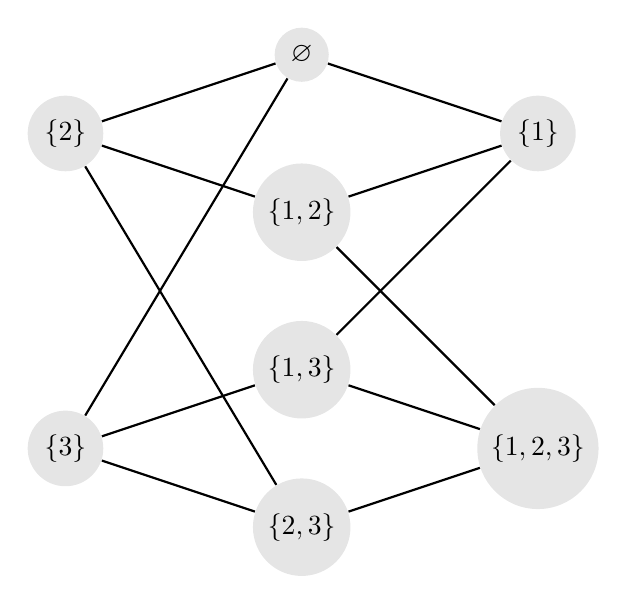
\begin{tikzpicture}
            \tikzstyle{vertex} = [circle, fill = black!10]
            \tikzstyle{edge}   = [-, thick]

            \node[vertex](v1)  at (0,1)  {$\{3\}$};
            \node[vertex](v2)  at (0,5)  {$\{2\}$};
            \node[vertex](v3)  at (3,0)  {$\{2,3\}$};
            \node[vertex](v4)  at (3,2)  {$\{1,3\}$};
            \node[vertex](v5)  at (3,4)  {$\{1,2\}$};
            \node[vertex](v6)  at (3,6)  {$\varnothing$};
            \node[vertex](v7)  at (6,1)  {$\{1,2,3\}$};
            \node[vertex](v8)  at (6,5)  {$\{1\}$};

            %%------------ Aristas ---------
            \draw[edge](v1)--(v3);
            \draw[edge](v1)--(v4);
            \draw[edge](v1)--(v6);
            \draw[edge](v2)--(v3);
            \draw[edge](v2)--(v5);
            \draw[edge](v2)--(v6);
            \draw[edge](v8)--(v4);
            \draw[edge](v8)--(v5);
            \draw[edge](v8)--(v6);
            \draw[edge](v7)--(v3);
            \draw[edge](v7)--(v4);
            \draw[edge](v7)--(v5);
          \end{tikzpicture}
        \end{center}

        %~~~~~~~~~~~~~~~~~~~~~~~~~~~~~~~~~~~~~~~~~~~ BL_4
        Gr\'afica representativa de $BL_4$:
        \begin{center}
          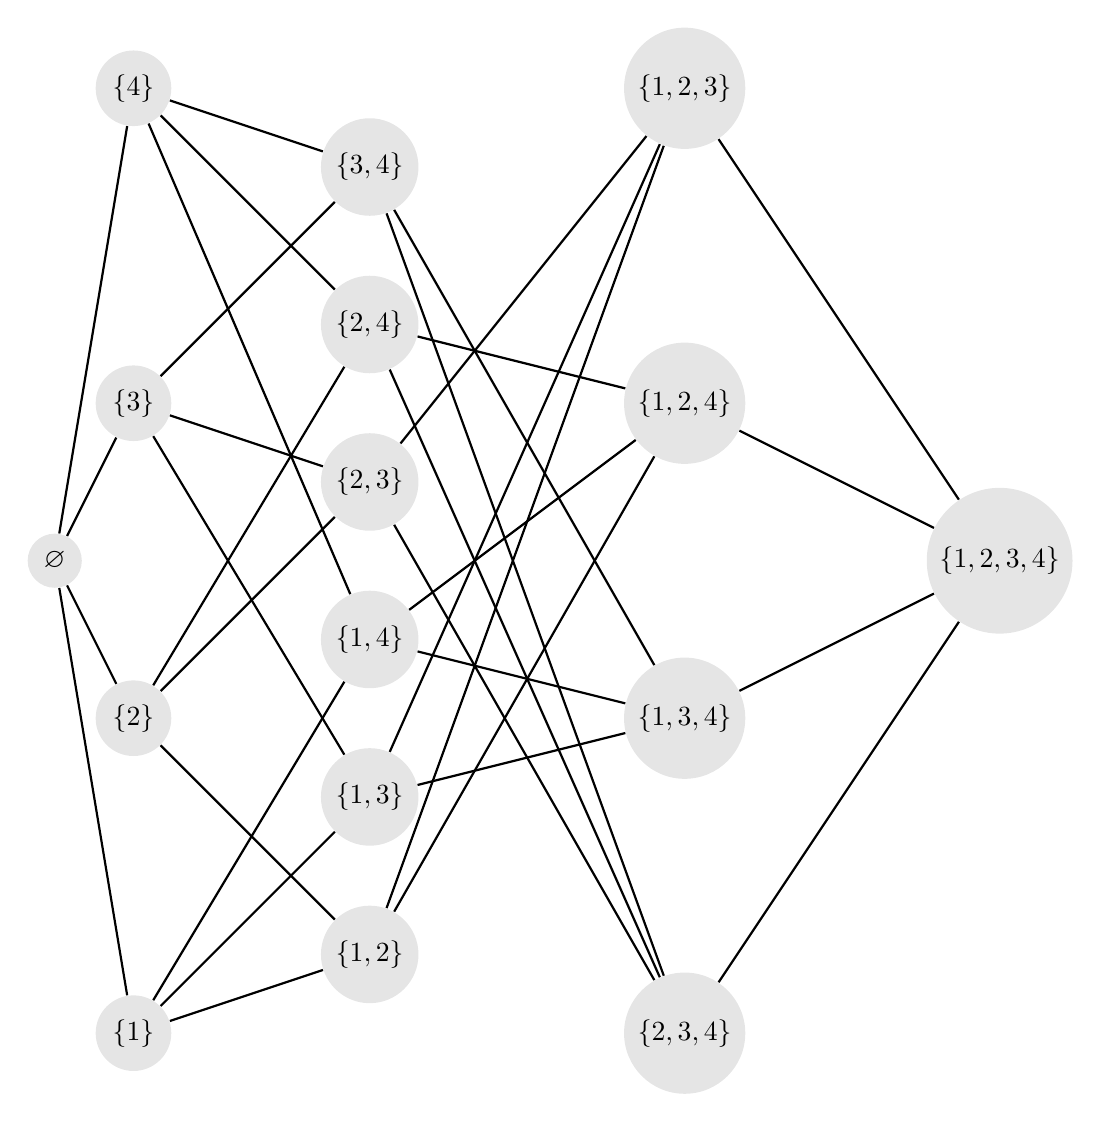
\begin{tikzpicture}
            \tikzstyle{vertex} = [circle, fill = black!10]
            \tikzstyle{edge}   = [-, thick]

            \node[vertex](v1)   at (0,6)    {$\varnothing$};
            \node[vertex](v2)   at (1,0)    {$\{1\}$};
            \node[vertex](v3)   at (1,4)    {$\{2\}$};
            \node[vertex](v4)   at (1,8)    {$\{3\}$};
            \node[vertex](v5)   at (1,12)   {$\{4\}$};
            \node[vertex](v6)   at (4,1)    {$\{1,2\}$};
            \node[vertex](v7)   at (4,3)    {$\{1,3\}$};
            \node[vertex](v8)   at (4,5)    {$\{1,4\}$};
            \node[vertex](v9)   at (4,7)    {$\{2,3\}$};
            \node[vertex](v10)  at (4,9)    {$\{2,4\}$};
            \node[vertex](v11)  at (4,11)   {$\{3,4\}$};
            \node[vertex](v12)  at (8,12)   {$\{1,2,3\}$};
            \node[vertex](v13)  at (8,8)    {$\{1,2,4\}$};
            \node[vertex](v14)  at (8,4)    {$\{1,3,4\}$};
            \node[vertex](v15)  at (8,0)    {$\{2,3,4\}$};
            \node[vertex](v16)  at (12,6)   {$\{1,2,3,4\}$};

            %%------------ Aristas ---------
            \draw[edge](v1)--(v2);
            \draw[edge](v1)--(v3);
            \draw[edge](v1)--(v4);
            \draw[edge](v1)--(v5);
            \draw[edge](v2)--(v6);
            \draw[edge](v2)--(v7);
            \draw[edge](v2)--(v8);
            \draw[edge](v3)--(v6);
            \draw[edge](v4)--(v9);
            \draw[edge](v3)--(v9);
            \draw[edge](v4)--(v7);
            \draw[edge](v5)--(v8);
            \draw[edge](v3)--(v10);
            \draw[edge](v4)--(v11);
            \draw[edge](v5)--(v11);
            \draw[edge](v5)--(v10);
            \draw[edge](v12)--(v6);
            \draw[edge](v12)--(v7);
            \draw[edge](v12)--(v9);
            \draw[edge](v13)--(v6);
            \draw[edge](v13)--(v8);
            \draw[edge](v14)--(v7);
            \draw[edge](v14)--(v8);
            \draw[edge](v15)--(v9);
            \draw[edge](v14)--(v11);
            \draw[edge](v13)--(v10);
            \draw[edge](v15)--(v11);
            \draw[edge](v15)--(v10);
            \draw[edge](v16)--(v12);
            \draw[edge](v16)--(v13);
            \draw[edge](v16)--(v14);
            \draw[edge](v16)--(v15);
          \end{tikzpicture}
        \end{center}
        \hfill $\square$

      %-------------------------- inciso (b) ---------------------
      \item Determine $|V_{BL_n}|$ y $|E_{BL_n}|$. (Justifique su respuesta).

        Veamos que la cantidad de v\'ertices es igual a la
        cantidad de subconjuntos que se pueden formar de
        la ret\'icula $BL_n$, esto es el conjunto potencia
        de $\{1, \dotsm, n\}$. Por lo que:
        \begin{center}
          $\abs{V_{BL_n}} = \abs{P \left(\{1, \dotsm, n\}\right)} = 2^{n}$
        \end{center}
        Mientras que es un tanto m\'as emp\'irica la forma en
        la que se obtiene la cardinalidad de $E_{BL_n}$,
        veamos la siguiente tabla con las primeras ret\'iculas:
        \begin{center}
          \begin{tabular}{|c|c|}
            \hline
            Valor de $n$ & $\#$ de aristas \\
            \hline
            $n = 1 \Rightarrow$ & $1$ arista \\
            \hline
            $n = 2 \Rightarrow$ & $4$ arista \\
            \hline
            $n = 3 \Rightarrow$ & $12$ arista \\
            \hline
            $n = 4 \Rightarrow$ & $32$ arista \\
            \hline
          \end{tabular}
        \end{center}
        N\'otese que:
        \begin{eqnarray*}
          1 \cdot 1 &= 1 \cdot 2^{1-1} =& 1\\
          2 \cdot 2 &= 2 \cdot 2^{2-1} =& 4\\
          3 \cdot 4 &= 3 \cdot 2^{3-1} =& 12\\
          4 \cdot 8 &= 4 \cdot 2^{4-1} =& 32
        \end{eqnarray*}
        Podemos deducir que $\abs{E_{BL_n}} = n \cdot 2^{n-1}$.

        \begin{center}
          \fbox{
            \begin{minipage}[b][1\height]%
              [t]{0.867\textwidth}
              En general, las ret\'iculas booleanas son $n$-regulares,
              pues para un $x \in V_{BL_{n - 1}}$ con $BL_{n - 1}$
              siendo $n$-regular, el  $BL_n$ tendr\'a a $x$ relacionado
              con al menos $n -1$ elementos (son con los que ya se
              relacionaba en $BL_{n - 1}$) y $x$ se relacionar\'a con
              el conjunto de tamaño $|x| + 1$ (el cu\'al s\'olo es uno,
              pues este es $x \cup \{n\}$) y concluimos que $BL_n$
              es $n$-regular, pues cada $x$ se relaciona con
              $(n - 1) + 1$ elemento.
          \end{minipage}}
        \end{center}

        Luego hay $n$ aristas por cada v\'ertice (los cu\'ales son
        $2^n$, como ya vimos) y por el inciso ($c$) tenemos que
        $BL_n$ es bipartita. Esto aunado al hecho de que es
        $n$-regular, nos da partes en $BL_n$ de igual
        cardinalidad. De lo anterior hay una cantidad de aristas
        igual a $n$ por cada una de las partes. Es decir:
        \begin{eqnarray*}
          |E_{BL_n}| &=& n \cdot \frac{2^n}{2}\\
          &=& n \cdot 2^{n - 1}
        \end{eqnarray*}


        \hspace*{4 cm} $\therefore\ \ \ \ \ \abs{V_{BL_n}} = 2^n
        \text{ y } |E_{BL_n}| = n \cdot 2^{n -1}$
        \hfill $\square$

      %-------------------------- inciso (c) ---------------------
      \item Demuestre que $BL_n$ es bipartita para cualquier $n \in \mathbb{Z}^+$.

      \begin{proof}

        Sea $A = \{1, \dotsm,n\}$ conjunto con $n \in \mathbb{Z}^+$. \\
        Veamos que podemos particionar nuestra $BL_n$ en los conjuntos
        $X$ y $Y$ de tal forma que $X$ contenga los subconjuntos de
        $BL_n$ tales que su cardinalidad es $2k$, donde $2k \in A$  y
        $Y$ tal que contenga los subconjuntos de $BL_n$ de cardinalidad
        $2k -1$, donde $2k -1 \in A$. \\

        Veamos qu\'e pasa cuando dos subconjuntos en $BL_n$ se relacionan,
        es decir, son adyacentes en $BL_n$.

        \begin{itemize}
          \item[-] Su diferencia sim\'etrica es $1$.
        \end{itemize}

        Dados dos subconjuntos en $BL_n$, uno de ellos debe tener cardinalidad
        $n+1$ o $n-1$ y el otro de cardinalidad $n$ tal que se cumple que uno
        de ellos es subconjunto del otro. \\

        Notemos que en $X$ est\'an todos los subconjuntos de cardinalidad par. \\
        Por tanto, la diferencia sim\'etrica entre cualesquiera 2 subconjuntos
        distintos en $X$ es:
        \begin{itemize}
        \item[-] A lo menos un conjunto de cardinalidad $2$.
        \end{itemize}
        De lo anterior, tenemos que ning\'un subconjunto en
        $X$ cumple ser adyacente mediante la definici\'on de $BL_n$.

        Ahora notemos que, en $Y$ est\'an todos los subconjuntos de
        $BL_n$  que tienen cardinalidad impar. \\
        Por lo tanto, la diferencia sim\'etrica en cualesquiera dos subconjuntos
        distintos en $Y$ es:

        \begin{itemize}
          \item[-] Al menos un conjunto de cardinalidad $2$.
        \end{itemize}

        Entonces tenemos que: $2k + 1 - (2k -1) = 2$ y como $Y$
        es un conjunto, no se tiene dos conjuntos iguales a los
        cuales relacionar. \\
        Por lo anterior y por la definici\'on de diferencia sim\'etrica, no existen dos conjuntos adyacentes en $Y$.

        \hspace*{3cm}  $\therefore$ \ \ \ $BL_n$ es bipartita en $X$ y $Y$, \textit{i.e.} $BL_n[X,Y]$
      \end{proof}
    \end{enumerate}

  %%%%%%%%%%%%%%%%%%%%%%%%%%%%%%%%% 5 %%%%%%%%%%%%%%%%%%%%%%%%%%%%%%%%%%%%%%%%%%%
  \item Sea $G[X, Y]$ una gr\'afica bipartita.
    \begin{enumerate}

      %-------------------------- inciso (a) ---------------------
      \item Demuestre que $\sum_{v \in X} d(v) = \sum_{v \in Y} d(v)$.
      \begin{proof}
        (Inducción sobre ${|Y|}$)

        Sea $G$ una gr\'afica bipartita $G[X,Y]$ y sea $r$ cualquier Entero tal que $|X|=r$.
        \begin{itemize}
          \item PASO BASE: ($n=1$)

            As\'i, tenemos $G[X,Y_{1}]$ donde $|X|=r$ y $|Y|=1$. \\
            Como $G$ es bipartita, todo v\'ertice de $X$ se relaciona con el \'unico elemento
            de $Y$. \\
            Por lo que $\sum_{v \in X}d(v) = r$ y el grado del \'unico v\'ertice
            en $Y$ es igual a $r$. \\
            Por lo tanto, $\sum_{v \in X}d(v) = r = \sum_{v \in Y_1}d(v)$. \\

          \item Hip\'otesis de Inducci\'on: ($n=k$)

            Supongamos que $G[X, Y_k]$ es una gr\'afica
            bipartita y $\sum_{v \in X}d(v) = \sum_{v \in Y_k}d(v)$. \\

          \item PASO INDUCTIVO: $(n=k+1)$

            Sea $G[X,Y_{k+1}]$ funci\'on bipartita. \\
            Demostraremos que $\sum_{v \in X} d(v) = \sum_{v \in Y_{k+1}}d(v)$.

            Por hip\'otesis de inducci\'on, tenemos que $\sum_{v \in X}d(v) = \sum_{v \in Y_k}d(v)$. Luego, si agregamos un v\'ertice a Y$_k$, tenemos que $|Y_k|+1 = |Y_{k+1}|$. \\
            Por defici\'on de gr\'afica bipartita, existir\'an v\'ertices de $X$ que son adyacentes
            con el nuevo v\'ertice en $Y$. \\
            Sea $q$ el número de nuevas relaciones entre $X$ y el nuevo v\'ertice en $Y$. \\
            Vemos que el grado del nuevo v\'ertice en $Y$ es igual a $q$. \\
            Entonces:
            $$\sum_{v \in X} d(v) = \sum_{v \in Y_k}d(v) + q =  \sum_{v \in Y_{k+1}}d(v)$$
        \end{itemize}

        Por lo tanto, para toda $G$ tenemos que $\sum_{v \in X}d(v) = \sum_{v \in Y}d(v)$.
        \end{proof}

      %-------------------------- inciso (b) ---------------------
      \item Demuestre que si $G$ es $k$-regular, con $k \ge 1$, entonces
        $|X| = |Y|$.

        \begin{proof}
          Dada $G$ una gr\'afica $k$-regular $G[X,Y]$ bipartita. \\
          Sabemos que por ser bipartita y $k$-regular, se cumple que:

          \begin{itemize}
            \item[-] Al menos $|V_G|=2$, pues una gr\'afica tiene como m\'inimo
            un elemento. Adem\'as, por ser bipartita debe relacionarse con al
            menos un elemento en la partici\'on ajena a ella misma.

            \item[-] Todos los v\'ertices tienen grado $k$.
          \end{itemize}

          En el caso mínimo $|V_G| = 2$, hay una relaci\'on entre
          dos v\'ertices (cada uno de ellos pertenecientes a su respectiva
          parte). \\
          Entonces, al ser $k$-regular, tenemos que el grado
          de estos v\'ertices es al menos $1$. \\
          Por lo tanto, $k \geq 1$.

          Ahora usando el resultado de $5$($a$), sabemos que:
          $$\sum_{v \in X} d(v) = \sum_{v \in Y} d(v)$$

          Como cada v\'ertice tiene grado $k$, podemos hacer lo siguiente:
          $$\abs{X} = \frac{\displaystyle \sum_{v \in X} d(v)}{k} \text{\hspace{0.3cm}
            \text{y} \hspace{0.3cm}} \abs{Y} = \frac{\displaystyle \sum_{v \in Y} d(v)}{k}$$

          As\'i, concluimos que:
          $$|X| = |Y|$$
        \end{proof}
    \end{enumerate}
\end{enumerate}

%%%%%%%%%%%%%%%%%%%%%%%%%%%%%%%% Extras %%%%%%%%%%%%%%%%%%%%%%%%%%%%%%%%%%%%%%%%
\subsection*{Puntos Extra}

\begin{enumerate}
<<<<<<< HEAD
  \item Sea $G = [X, Y]$ una gr\'afica bipartita con $|X| = r$ y $|Y| = s$.

    \begin{enumerate}
      \item Demuestre que $|E| \le rs$.
        %---------------------------------------------------------------------------------------------
        \begin{proof}
          (Inducción sobre $|Y|$)

          Sea $r$ cualquier Entero tal que $|X|=r$.
          \begin{itemize}
            \item PASO BASE: $(n = 1)$

              Sea $G(V_1, E_1)$ tal que $G[X,Y]$, con $|Y|=1$. \\
              Se sigue por vacuidad que, MAX$\{|E_1|\}=r$ (pues todo elemento de $X$ solo se puede relacionar al \'unico v\'ertice en $Y$). \\

            \item Hip\'otesis de inducci\'on: ($n = k$)

              Supongamos que existe $G(V_k, E_k)$ tal que $G[X,Y]$, con $|X|=r$ y $|Y|= k$. \\ Entonces: $MAX\{|E_k|\} = rk$. \\

            \item PASO INDUCTIVO: ($n=k+1$)

              Sea $G(V_{(k+1)}, E_{(k+1)})$ tal que $G[X,Y]$, con $|X|=r$ y $|Y|=k+1$. \\
              Entonces: MAX$\{|E_{(k+1)}|\} = r(k+1)$. \\

              Por Hip\'otesis de inducci\'on, $G(V_k, E_k)$ tal que $G[X,Y]$, con $|X|=r$ y $|Y|=k$,
              por lo que MAX$\{|Ek|\}=rk$. Agregando un v\'ertice a $Y$, tenemos que $|V(k+1)|$ = 1 + $|Vk|$. As\'i, se tiene que MAX$\{|E(k+1)|\}$ = MAX$\{|Ek|\} + k$ (donde $k$ son las nuevas relaciones entre el v\'ertice que se agreg\'o y todos los v\'ertices de $X$). \\
              Entonces:
              $$\text{MAX}\{|Ek|\} + k = rk + r = r(k+1)$$

              Por lo anterior, tenemos que MAX$\{|E(k+1)|\} = r(k+1)$.
          \end{itemize}

          Por lo tanto, para toda $G(V, E)$ si $G[X,Y]$ con $|X|=r$ y $|Y|=s$, MAX$\{|E|\} = rs$.
        \end{proof}

      %---------------------------------------------------------------------------------------------
      \item Deduzca que $|E| \le \frac{|V|^2}{4}$.
        %-----------------------------------------------------------------------------------------------
        \begin{proof}
          Demostraremos que $rs \leqslant (|V|^2)/4$. \\

          Sabemos que para toda gr\'afica $G[X,Y]$, $|X|=r$ y $|Y|=s$ con $r,s$ que pertenecen a los Enteros. \\
          Por un Teorema de C\'alculo ($x^2 > 0$), $0 \leqslant (r-s)^2  \Longrightarrow 0   \leqslant r^2 + s^2 -2rs \Longrightarrow 2rs \leqslant r^2 + s^2 \Longrightarrow 4rs \leqslant r^2 + s^2 + 2rs \Longrightarrow 4rs \leqslant (r+s)^2 \Longrightarrow rs \leqslant ((r+s)^2)/4 $ y $r+s = |X|+|Y|$ por lo que por definición de particion $|X| + |Y| = |V|  \Longrightarrow (|V|^2)/4$ por inciso $(a)$ tenemos que:  $|E|\leqslant rs \leqslant (|V|^2)/4$
           por lo tanto $ |E|\leqslant (|V|^2)/4 $

        \end{proof}
      %-----------------------------------------------------------------------------------------------
      \item Describa a las gr\'aficas bipartitas que cumplen la igualdad en el
      inciso anterior. Justifique su respuesta.
        %------------------------
        SOLUCION

        Debemos ver donde se cumple la igualdad $|E|= (|V|^2)/4$

        Sea $|V|= |X| + |Y| = r+s \Longrightarrow$ por la demostración del inciso del inciso $(b)$ y $(a)$ tenemos que si $0\leqslant(r-s)^2 \Longrightarrow |E|\leqslant rs \leqslant (|V|^2)/4 \Longrightarrow$ si $0=(r-s)^2 \Longrightarrow 0=r-s \Longrightarrow s=r \Longrightarrow rs=(|V|^2)/4 $ y si G es una gráfica bipartita completa $\Longrightarrow |E|=rs=(|V|^2)/4$ por lo tanto, si las particiones de la gráfica tienen el mismo número de elementos y tambien la gráfica es bipartita completa se cumple la desigualdad $|E|= (|V|^2)/4$
        \newpage
        Ejemplo:
        %\end{itemize}
        \begin{figure}[ht!]
            \centering
                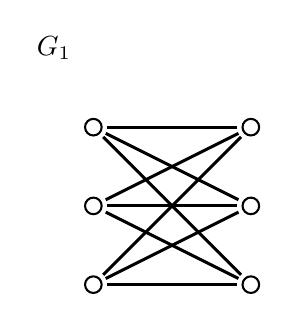
\begin{tikzpicture}
                    \node (0) [vertex,label=180:] at (0,0){};
                    \node (1) [vertex,label=180:] at (0,-1){};
                    \node (2) [vertex,label=180:] at (0,-2){};
                    \node (3) [vertex,label=180:] at (2,0){};
                    \node (4) [vertex,label=180:] at (2,-1){};
                    \node (5) [vertex,label=180:] at (2,-2){};

                     \draw [edge] (0) to (3);
                     \draw [edge] (0) to (4);
                     \draw [edge] (0) to (5);
                     \draw [edge] (1) to (3);
                     \draw [edge] (1) to (4);
                     \draw [edge] (1) to (5);
                     \draw [edge] (2) to (3);
                     \draw [edge] (2) to (4);
                     \draw [edge] (2) to (5);

                    \node (L) at (-0.5,1){$G_1$}; %nobre de la grafica
                \end{tikzpicture}
        \end{figure}
        $rs=9$

        $|E|=9$

        $|V|= 9 \Longrightarrow |V|^2/4 = 36/4 = 9$
        %------------------------
    \end{enumerate}
=======
\item Sea $G = [X, Y]$ una gr\'afica bipartita con $|X| = r$ y $|Y| = s$.
  \begin{enumerate}
  \item Demuestre que $|E| \le rs$.
%---------------------------------------------------------------------------------------------
\begin{proof}
  (Inducción sobre $|Y|$) 
  
  Sea r cualquier Entero tal que $|X|=r$
  
  Paso base $(n = 1)$: Sea G($V_1$,$E_1$): $G[X,Y]$ donde $|Y|=1\Longrightarrow$  se sigue por vacuidad que MAX$\{|E_1|\}$=r (ya que todo elemento de X solo se puede relacionar al unico vértice  en Y). 
  
  Hipótesis de inducción($ n = k$): Supongamos que existe G(V$_k$, E$_k$): G[X,Y] tal que $|X|=r$ y $|Y|= k$ $\Longrightarrow$ MAX$\{|E_k|\} = rk$
  
  Pd) (para n=k+1): G(V$_{(k+1)}$,E$_{(k+1)}$): G[X,Y] tal que $|X|=r$ y $|Y|=k+1 \Longrightarrow$ 
  MAX$\{|E_{(k+1)}|\} = r(k+1)$
  
  Dem
  
  Por Hipótesis de inducción si G(V$_k$,E$_k$): G(X,Y) tal que $|X|=r$ y $|Y|=k$ por lo que 
  el MAX$\{|Ek|\}=rk $ agregando un vertice a Y $\Longrightarrow$ definimos $|V(k+1)|$ = 1 + $|Vk|$ por lo que el MAX$\{|E(k+1)|\}$ = MAX$\{|Ek|\} + $ k (donde k son las nuevas relaciones entre el vertice que se agrego y todos los vertices de X) $\Longrightarrow$ MAX$\{|Ek|\} + $ k $= rk +r = r(k+1)$
  
  por lo tanto el MAX$\{|E(k+1)|\} = r(k+1)$.
  
  Por lo tanto, para toda G(V,E) si G[X,Y]: $|X|=r$ y $|Y|=s \Longrightarrow$ MAX$\{|E|\} =$ rs
  \end{proof}
%---------------------------------------------------------------------------------------------
  \item Deduzca que $|E| \le \frac{|V|^2}{4}$.
%-----------------------------------------------------------------------------------------------
\begin{proof}
  PD. rs $ \leqslant (|V|^2)/4$
  
  Sabemos que para toda gráfica G$=[X,Y]: |X|=r$ y $|Y|=s \Longrightarrow$ (por teo. cálculo $x^2 > 0$) sean cualesquiera r,s que pertenecen a los Enteros  $\Longrightarrow  0 \leqslant (r-s)^2  \Longrightarrow 0   \leqslant r^2 + s^2 -2rs \Longrightarrow 2rs \leqslant r^2 + s^2 \Longrightarrow 4rs \leqslant r^2 + s^2 + 2rs \Longrightarrow 4rs \leqslant (r+s)^2 \Longrightarrow rs \leqslant ((r+s)^2)/4 $ y $r+s = |X|+|Y|$ por lo que por definición de particion $|X| + |Y| = |V|  \Longrightarrow (|V|^2)/4$ por inciso $(a)$ tenemos que:  $|E|\leqslant rs \leqslant (|V|^2)/4$
   por lo tanto $ |E|\leqslant (|V|^2)/4 $ 
  
  \end{proof}
%-----------------------------------------------------------------------------------------------

  \item Describa a las gr\'aficas bipartitas que cumplen la igualdad en el
    inciso anterior. Justifique su respuesta.
%------------------------
SOLUCION

Debemos ver donde se cumple la igualdad $|E|= (|V|^2)/4$

Sea $|V|= |X| + |Y| = r+s \Longrightarrow$ por la demostración del inciso del inciso $(b)$ y $(a)$ tenemos que si $0\leqslant(r-s)^2 \Longrightarrow |E|\leqslant rs \leqslant (|V|^2)/4 \Longrightarrow$ si $0=(r-s)^2 \Longrightarrow 0=r-s \Longrightarrow s=r \Longrightarrow rs=(|V|^2)/4 $ y si G es una gráfica bipartita completa $\Longrightarrow |E|=rs=(|V|^2)/4$ por lo tanto, si las particiones de la gráfica tienen el mismo número de elementos y tambien la gráfica es bipartita completa se cumple la desigualdad $|E|= (|V|^2)/4$


Ejemplo:
%\end{itemize}
%\begin{center}
\begin{figure}[ht!]                                                             
  \centering
  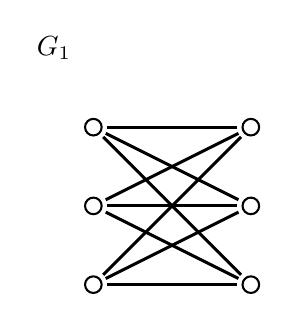
\begin{tikzpicture} 
    \node (0) [vertex,label=180:] at (0,0){};
    \node (1) [vertex,label=180:] at (0,-1){};   
    \node (2) [vertex,label=180:] at (0,-2){};   
    \node (3) [vertex,label=180:] at (2,0){};   
    \node (4) [vertex,label=180:] at (2,-1){};   
    \node (5) [vertex,label=180:] at (2,-2){};
    
    \draw [edge] (0) to (3); 
    \draw [edge] (0) to (4); 
    \draw [edge] (0) to (5); 
    \draw [edge] (1) to (3); 
    \draw [edge] (1) to (4); 
    \draw [edge] (1) to (5); 
    \draw [edge] (2) to (3); 
    \draw [edge] (2) to (4); 
    \draw [edge] (2) to (5); 
    
    \node (L) at (-0.5,1){$G_1$}; %nobre de la grafica 
  \end{tikzpicture}
\end{figure}
%\end{center}

Obsérvese que $rs=9$, $|E|=9$, y $|V| = 9$ implica que $|V|^2/4 = 36/4 = 9$.
%------------------------
>>>>>>> Adrian-Aguilera
  \end{enumerate}
\end{document}
